\documentclass[twocolumn]{article}
\usepackage{graphicx}
\usepackage{fullpage}

\title{Exponential function approximation}
\author{Jens Høj Christiansen}
\begin{document}

\maketitle

\section{Exponential function}

We have the exponential function, which is defined by

$$\exp(x) = \sum_k \frac{x^k}{k!} = 1 + x + \frac{x^2}{2} + \frac{x^3}{6} + ...$$

A quick and dirty approximation to this function is

$$\exp(x) = 1+x\left(1+\frac{x}{2}\left(1+\frac{x}{3}\left(1+\frac{x}{4}\left(1+\frac{x}{5}\left(1+\frac{x}{6}\left(1+\frac{x}{7}\left(1+\frac{x}{8}\left(1+\frac{x}{9}\left(1+\frac{x}{10}\right) \right) \right) \right) \right) \right) \right) \right) \right)$$

Which is an expansion of the exponential function. It is easily seen, if the parenthesies are calculated.

Plots of the two functions are found in figure 1.

\begin{figure}[h]
    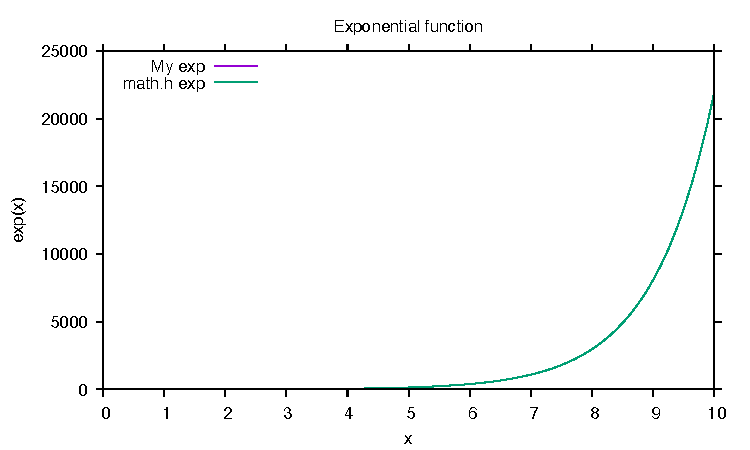
\includegraphics{plot.gnuplot.pdf}
    \caption{Exponential functions}
    \label{fig:Gnuplot}
\end{figure}

From which it is evident that the quick and dirty implementation works well in this interval.

\end{document}